\documentclass[11pt, a4paper]{article}
\usepackage{fullpage}
\usepackage[USenglish]{babel}
\usepackage{graphicx} 
\usepackage[small,bf,hang]{caption2}
\usepackage{hyperref}
\hypersetup{
    colorlinks,
    citecolor=black,
    filecolor=black,
    linkcolor=black,
    urlcolor=black
}

\title{Master Thesis -  Security Aspects in Virtual Networks\\ \textbf{SITREP 11}}
\author{\textbf{Laurent De Wilde} \\ Master of Science in the Applied Computer Science \\ Vrije Universiteit Brussel}
\date{March 23, 2015}

\begin{document}
\maketitle

\section*{Work done}

This is an overview of the work performed in the past week:
\begin{itemize}
\item Installed Snort IDS on an Ubuntu VM running on Hyper-V as shown on the figure below. The switch port of the Snort VM is now the destination, meaning it ``sees'' all the traffic on the other Hyper-V VM's as well as the traffic that is sent to the Hyper-V host. As will turn out later, Snort is also able to ``see'' traffic from and to the Xen virtual network.
\begin{figure}[h]
    \centering
    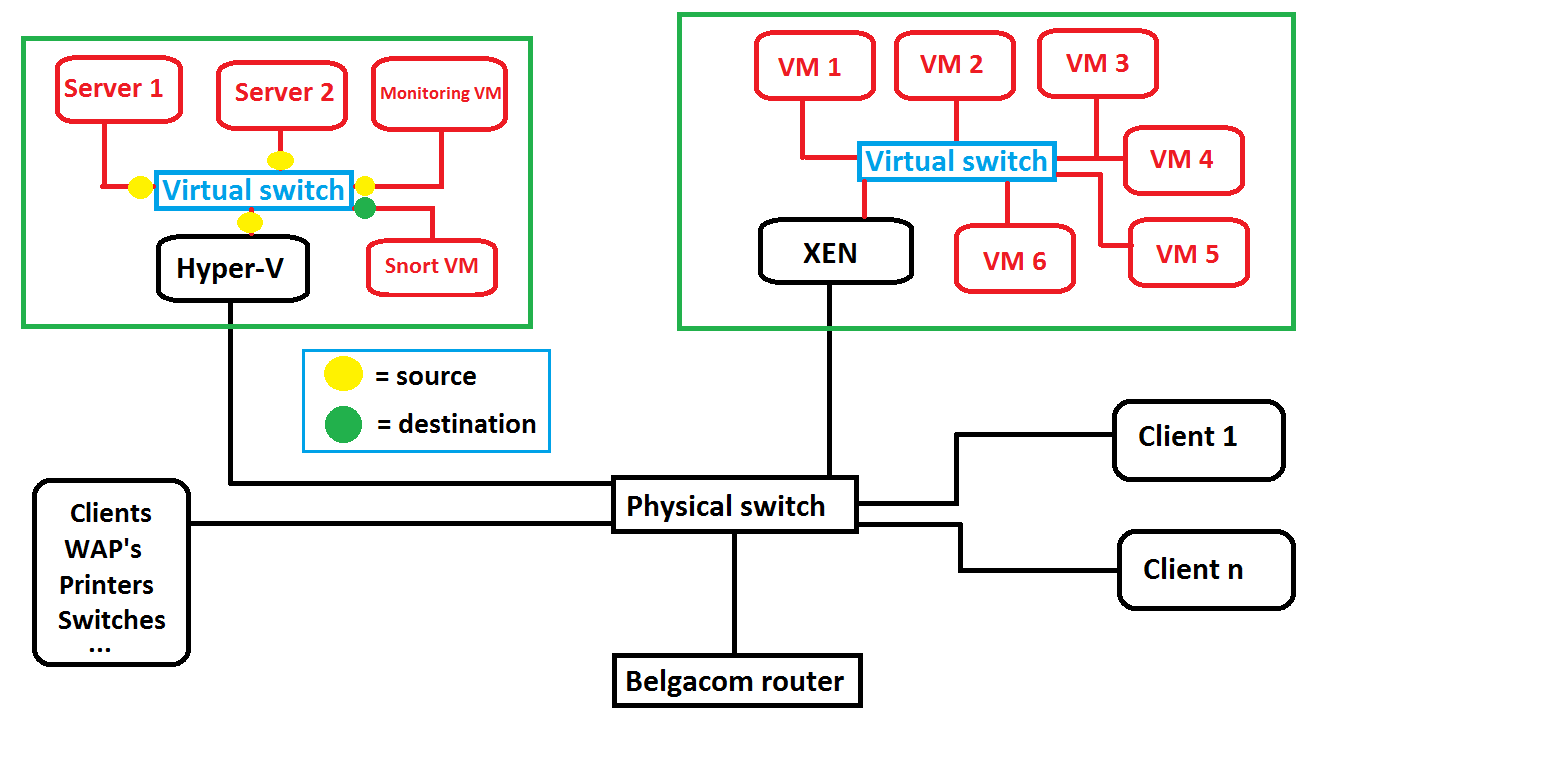
\includegraphics[width=1\textwidth]{Network.png}
   \caption{The modified and network setup.}
\end{figure}
\item Tested the VM to see if it is indeed capturing / sniffing network traffic. Therefore, I used ``tcpdump''. This was indeed the case. So this means that all traffic to and from the virtual Hyper-V network is picked up by the SnortVM and therefore also by Snort itself as it will turn out later.
\begin{figure}[h]
    \centering
    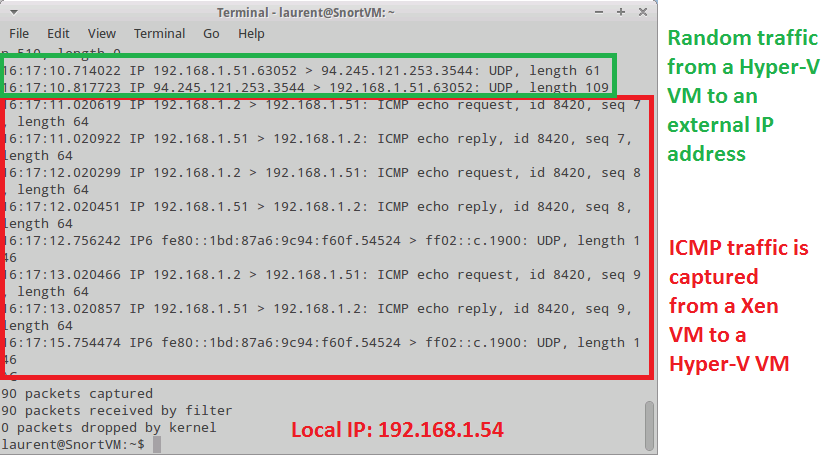
\includegraphics[width=1\textwidth]{Snort_1.png}
   \caption{Traffic is captured from a Hyper-V VM to an external IP address and from a Xen VM to a Hyper-V VM by the sniffer (tcpdump).}
\end{figure}
\begin{figure}[h]
    \centering
    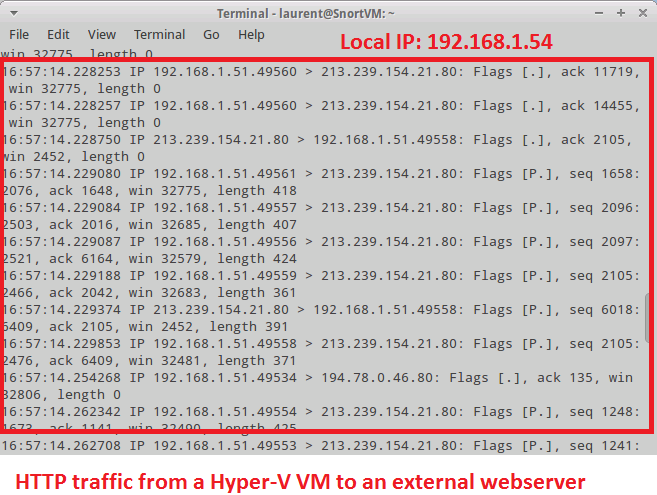
\includegraphics[width=0.85\textwidth]{Snort_2.png}
   \caption{Traffic is captured from a Xen VM to a Hyper-V VM by the sniffer (tcpdump).}
\end{figure}
\clearpage
\item Tested Snort for the correct working (added PING rules) as can be seen in the figure below. It turns out that Snort is indeed capable of detecting intrusions on the Hyper-V virtual network.
\begin{figure}[h]
    \centering
    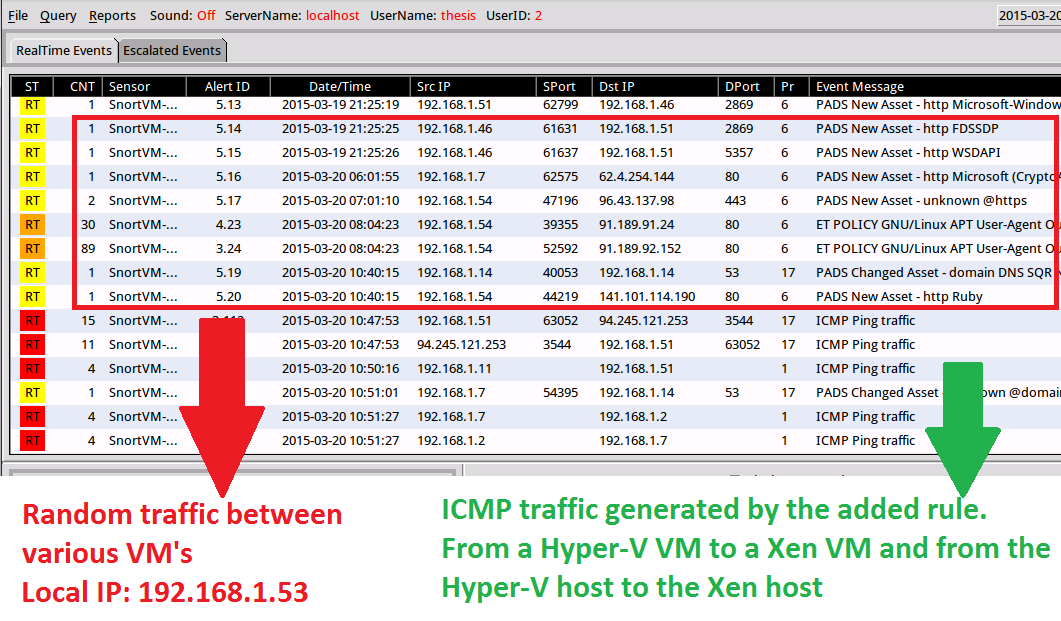
\includegraphics[width=1\textwidth]{Snort_3.png}
   \caption{Snort is indeed picking up traffic / intrusions on the Hyper-V virtual network and reports so.}
\end{figure}
\item However, Snort is only picking up intrusions on the Hyper-V network including the Hyper-V host. Thus, intrusions on the Xen virtual network are not detected, because those VM's resides on a seperate virtual switch.

So I wanted a way to also detect malicious activity on the Hyper-V network with the SnortVM running on a seperate virtual network.

Since I'm using in-kernel bridging for the virtual Xen switch, my initial idea was to snif the bridged interface (since all traffic - also between VM's - passes through this interface) and copy all the packets to another, physical interface set in promiscious mode. From there, I could then forward the packets to the Hyper-V network.

However, it is not possible to forward packets on an interface that is in promiscious mode. So instead of making a copy of the bridged interface, the only solution was to make a copy of the packets on each virtual interface connected to the vSwitch.

This solution works fine as illustrated in the following screenshots.
\end{itemize}
\clearpage
\begin{figure}[h]
    \centering
    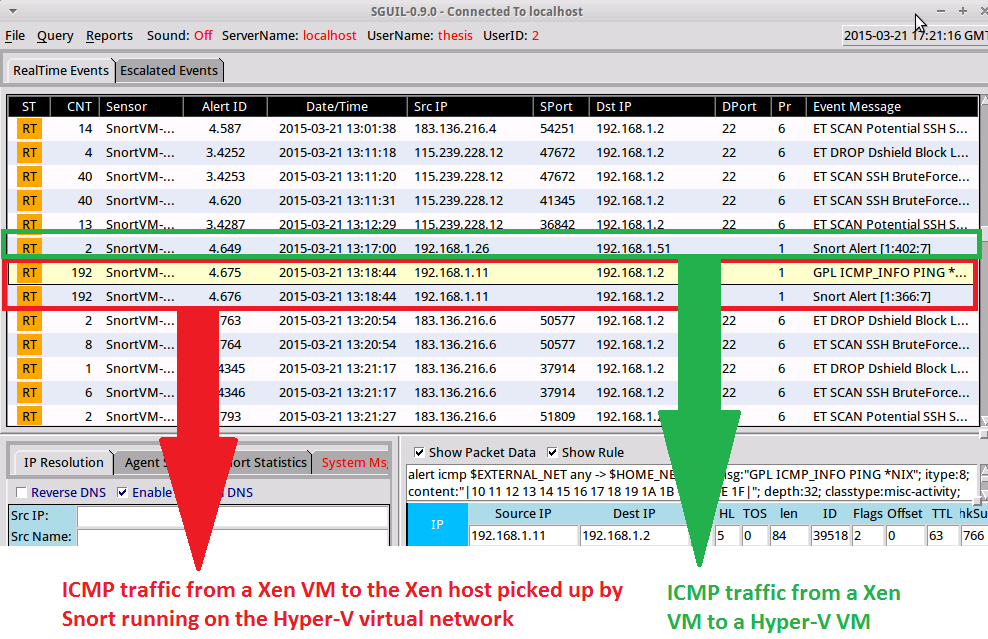
\includegraphics[width=1\textwidth]{Snort_4.png}
   \caption{Traffic / intrusions between a Xen VM and a Xen host as well as intrusions between a Xen VM to the Hyper-V host.}
\end{figure}
\begin{figure}[h]
    \centering
    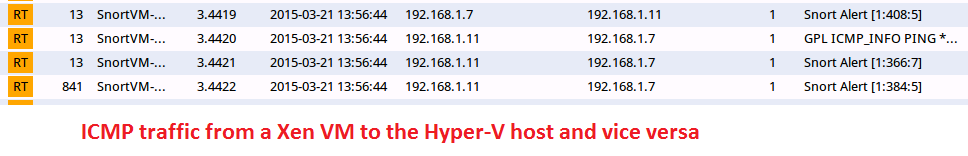
\includegraphics[width=1\textwidth]{Snort_5.png}
   \caption{From a Xen VM to the Hyper-V host.}
\end{figure}
\begin{figure}[h]
    \centering
    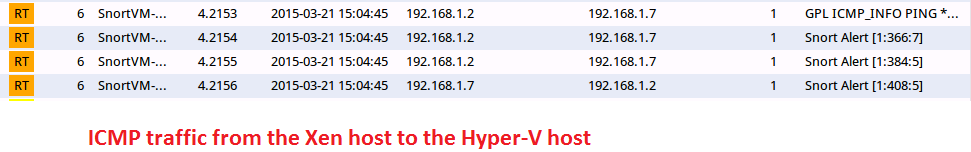
\includegraphics[width=1\textwidth]{Snort_6.png}
   \caption{Intrusions between the two hosts of both virtual networks.}
\end{figure}
\begin{figure}[h]
    \centering
    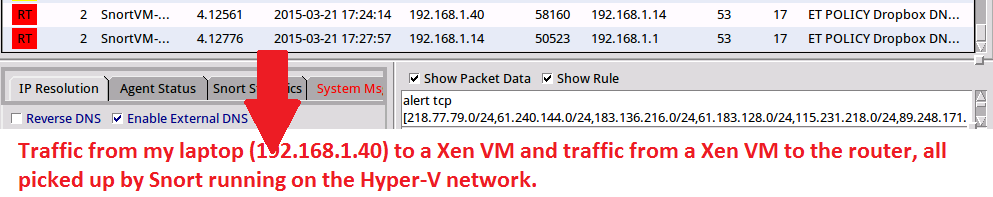
\includegraphics[width=1\textwidth]{Snort_17.png}
   \caption{Traffic / intrusions from a client to a Xen VM (Xen virtual network) picked up by Snort running on the Hyper-V network.}
\end{figure}
\begin{figure}[h]
    \centering
    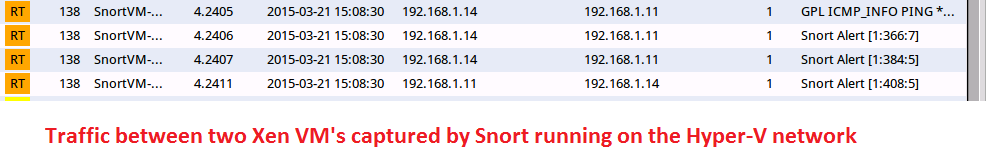
\includegraphics[width=1\textwidth]{Snort_8.png}
   \caption{Traffic / intrusions between two Xen VM's (inside the Xen virtual network) picked up by Snort running on the Hyper-V network.}
\end{figure}
\clearpage
\textbf{So to summarize, the following is possible / is achieved regarding intrusions:}
\begin{itemize}
\item Detecting intrusions between two VM's running on the Hyper-V virtual network.
\item Detecting intrusions between a VM running on the Hyper-V virtual network and the Xen virtual network and vice versa.
\item Detecting intrusions between two VM's running on the Xen virtual network.
\item Detecting intrusions between the Xen host and Hyper-V host and vice versa.
\end{itemize}
\section*{Planning}
 



\section*{Problems}



\section*{Issues}

\begin{figure}[h]
    \centering
    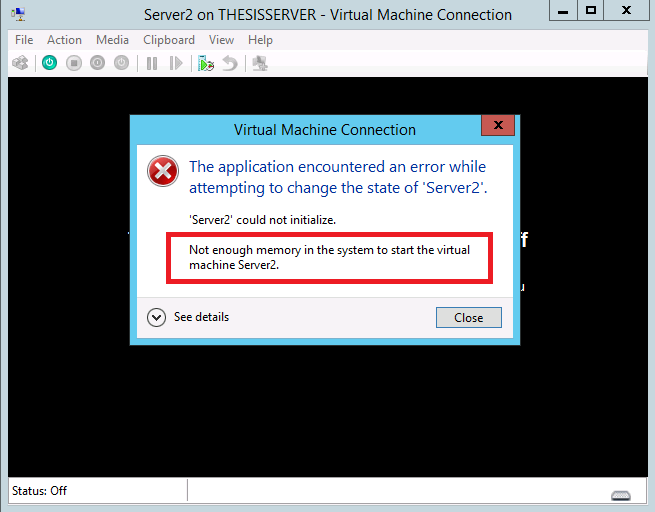
\includegraphics[width=1\textwidth]{Mem.png}
   \caption{Running two Windows 7 VM's with each 1GB of RAM is not possible with Snort running on the same host with 8GB of RAM. Only one Windows 7 VM is able to run with a Snort VM on the same Hyper-V host with 8GB of RAM.}
\end{figure}
\begin{figure}[h]
    \centering
    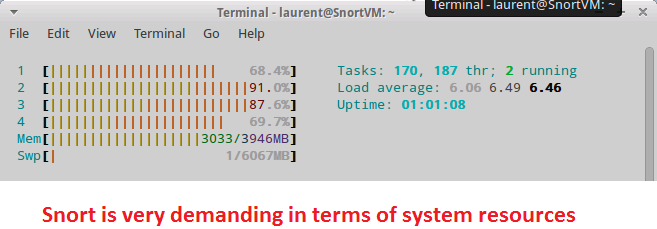
\includegraphics[width=1\textwidth]{Mem_2.png}
   \caption{Snort uses a lot of system resources.}
\end{figure}
\clearpage
\section*{Assistance}

Is it possible, before the Easter holidays, to reserve another server that I can experiment with for my MA thesis? The current server with Hyper-V installed on is a single boot installation, but for future work, I'll need a dual boot system and I would rather not format the current pizza server.

Any type of server (tower or pizza) is OK.


\end{document}